% Options for packages loaded elsewhere
\PassOptionsToPackage{unicode}{hyperref}
\PassOptionsToPackage{hyphens}{url}
%
\documentclass[
]{article}
\usepackage{amsmath,amssymb}
\usepackage{lmodern}
\usepackage{iftex}
\ifPDFTeX
  \usepackage[T1]{fontenc}
  \usepackage[utf8]{inputenc}
  \usepackage{textcomp} % provide euro and other symbols
\else % if luatex or xetex
  \usepackage{unicode-math}
  \defaultfontfeatures{Scale=MatchLowercase}
  \defaultfontfeatures[\rmfamily]{Ligatures=TeX,Scale=1}
\fi
% Use upquote if available, for straight quotes in verbatim environments
\IfFileExists{upquote.sty}{\usepackage{upquote}}{}
\IfFileExists{microtype.sty}{% use microtype if available
  \usepackage[]{microtype}
  \UseMicrotypeSet[protrusion]{basicmath} % disable protrusion for tt fonts
}{}
\makeatletter
\@ifundefined{KOMAClassName}{% if non-KOMA class
  \IfFileExists{parskip.sty}{%
    \usepackage{parskip}
  }{% else
    \setlength{\parindent}{0pt}
    \setlength{\parskip}{6pt plus 2pt minus 1pt}}
}{% if KOMA class
  \KOMAoptions{parskip=half}}
\makeatother
\usepackage{xcolor}
\IfFileExists{xurl.sty}{\usepackage{xurl}}{} % add URL line breaks if available
\IfFileExists{bookmark.sty}{\usepackage{bookmark}}{\usepackage{hyperref}}
\hypersetup{
  hidelinks,
  pdfcreator={LaTeX via pandoc}}
\urlstyle{same} % disable monospaced font for URLs
\usepackage[margin=1in]{geometry}
\usepackage{longtable,booktabs,array}
\usepackage{calc} % for calculating minipage widths
% Correct order of tables after \paragraph or \subparagraph
\usepackage{etoolbox}
\makeatletter
\patchcmd\longtable{\par}{\if@noskipsec\mbox{}\fi\par}{}{}
\makeatother
% Allow footnotes in longtable head/foot
\IfFileExists{footnotehyper.sty}{\usepackage{footnotehyper}}{\usepackage{footnote}}
\makesavenoteenv{longtable}
\usepackage{graphicx}
\makeatletter
\def\maxwidth{\ifdim\Gin@nat@width>\linewidth\linewidth\else\Gin@nat@width\fi}
\def\maxheight{\ifdim\Gin@nat@height>\textheight\textheight\else\Gin@nat@height\fi}
\makeatother
% Scale images if necessary, so that they will not overflow the page
% margins by default, and it is still possible to overwrite the defaults
% using explicit options in \includegraphics[width, height, ...]{}
\setkeys{Gin}{width=\maxwidth,height=\maxheight,keepaspectratio}
% Set default figure placement to htbp
\makeatletter
\def\fps@figure{htbp}
\makeatother
\setlength{\emergencystretch}{3em} % prevent overfull lines
\providecommand{\tightlist}{%
  \setlength{\itemsep}{0pt}\setlength{\parskip}{0pt}}
\setcounter{secnumdepth}{5}
\ifLuaTeX
  \usepackage{selnolig}  % disable illegal ligatures
\fi

\author{}
\date{\vspace{-2.5em}}

\begin{document}

{
\setcounter{tocdepth}{2}
\tableofcontents
}
\hypertarget{discrete-time-model}{%
\subsubsection{Discrete Time Model}\label{discrete-time-model}}

We formalized the learning problem that participants face in our experiments as a form of Bayesian concept learning {[} @goodman2008rational;@tenenbaum1999bayesian{]}, represented graphically in Fig. X. The goal is to learn a concept \(\theta\), which is a set of probabilities for independent binary features \(\theta_{1,2,..,n}\), where n is the number of features. Over the course of a block, the learner receives information about \(\theta\) by observing exemplars \(y\): instantiations of \(\bar{\theta}\), where each feature \(y_{1,2,..,n}\) is either on or off. Each feature \(\theta_i\) and its corresponding exemplar \(y_i\) form a Beta-Bernoulli process:
\begin{eqnarray}
p(\theta_i) \sim Beta(\alpha_i,\beta_i) \\
p(y_i|\theta_i) \sim Bernoulli(\theta_i)
\end{eqnarray}
Since the features are independent, this relationship holds for the entire concept \(\theta\). In previous work, two information-theoretic quantities, surprisal and Kullback-Leibler (KL) divergence, resulting from the stimulus were shown to be linked to looking behavior {[}@kidd2012goldilocks; @poli2020infants{]}. Surprisal, calculated as \(-log(p(y|\theta))\), intuitively refers to how surprising a stimulus \(y\) is given the model's beliefs about \(\theta\) - the intuition that surprising events should result in longer looking times has served as a foundational assumption in developmental psychology. KL-divergence measures how much a model needs to change to accommodate a new stimulus \(y\), and describes a distance between the model before and after an observation, in is defined in our case as \(\sum_{x \in X}{p(\theta = x|y)\frac{p(\theta = x|y)}{p(\theta = x)}}\). If an observation causes a large change, we speculated that a proportionally long looking time is necesssary to integrate the new information.

\hypertarget{continuous-time-model}{%
\subsubsection{Continuous Time Model}\label{continuous-time-model}}

However, to model the time course of attention, we did not want to assume that stimuli are encoded perfectly and instantaneously. Instead, we suggest that participants gather repeated noisy samples \(\bar{z}\) from the exemplars. For any sample \(z\) from an exemplar \(y\) there is a small probability \(\epsilon\) to misperceive the feature as off when it was actually on, and vice versa.
Therefore, by making noisy observations \(\bar{z}\), the learner obtains information about the true identity of the exemplar \(y\), and by extension, about the concept \(\bar{theta}\). By Bayes' rule:
\begin{eqnarray}
P(\theta|\bar{z}) &= p(\bar{z}|y) p(y|\theta) p(\theta) / p(\bar{z})
\end{eqnarray}
where \(p(\bar{z}|y_i)\) is fully described by \(\epsilon\), and \(p(y|\theta)\) by Bernoulli processes as in Eq. 2.

\begin{figure}[H]

{\centering 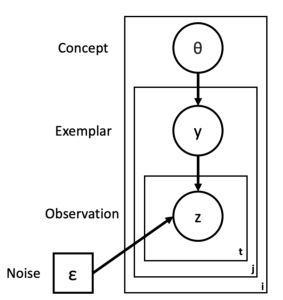
\includegraphics{02_model_files/figure-latex/plate_diagram-1} 

}

\caption{Graphical representation of our model. Circles indicate random variables. The squares indicate fixed model parameters.}(\#fig:plate_diagram)
\end{figure}

\hypertarget{sampling}{%
\paragraph{Sampling}\label{sampling}}

The formulation of the model in continuous time allows us to do two things: First, we can explicitly model the learner's decision on when to stop sampling by asking the model to decide, after every sample \(z\), whether it wants to continue sampling from the same stimulus or not. This is in contrast to the discrete time models presented here and in previous work (Kidd et al., 2012; Poli et al., 2020), where we can only link information-theoretic measures to looking data, but not provide a mechanism for how these measures could control moment-to-moment sampling decisions. Second, a consequence of making a decision at every time step is that we can study the behavior of another information-theoretic measure: the expected information gain (EIG). EIG is commonly used in rational analyses of information-seeking behavior - that is to assess whether information-seeking is optimal with respect to the learning task {[}@markant2012does;@oaksford1994rational{]}. Importantly, EIG is a forward-looking measure that considers the potential for learning from the next sample. Since discrete time models operate on the level of a whole stimulus, rather than individual samples, EIG would look forward to the next stimulus in these models, rather than the next sample, and therefore not be able to capture the decision of whether to keep looking. EIG to describe looking time is therefore only possible in the continuous time models.

We compute EIG by weighing the information gain from each possible next observation by the probability of that observation. We defined information gain as the KL-divergence between the hypothetical posterior after observing a sample \(z_{t+1}\) and the current posterior:
\begin{eqnarray}
EIG(z_{t+1}) = \sum_{z_{t+1} \in [0,1]} p(z_{t+1}|\theta_t) * KL(\theta_{t+1}, p(\theta_t))
\end{eqnarray}
Finally, to get actual sampling behavior from the model, it has to convert EIG into a binary decision about whether continue looking at the current sample, or to advance to the next trial. The model does so using a luce choice between the EIG from the next sample and a constant EIG from looking away.
\begin{eqnarray}
p(look) = \frac{EIG(z_{t+1})}{EIG(z_{t+1})+EIG(world)}
\end{eqnarray}
We also studied the behavior of the model when replacing EIG with continuous time versions of the other linking hypotheses, surprisal and KL-divergence between the posterior \(p(\theta_t)\) and the prior \(p(\theta_{t-1})\).

\end{document}
